% =============================================================================
% NL2Semantic2SQL: A Cross-Domain Framework for Natural Language to SQL over
% Geospatial and Enterprise Data Warehouses
% Initial-review LaTeX draft (single column, generic article class).
% Final update: GIS Spatial/Robustness split (p=0.0072/p=0.0156), DIN-SQL on GIS 100q (Full vs DIN p=0.0213/p=0.0078), BIRD 495q (EX=0.501), CIs, token cost.
% =============================================================================
\documentclass[11pt]{article}

\usepackage[margin=1in]{geometry}
\usepackage{times}
\usepackage{amsmath,amssymb}
\usepackage{graphicx}
\usepackage{booktabs}
\usepackage{multirow}
\usepackage{caption}
\usepackage{subcaption}
\usepackage{enumitem}
\usepackage{url}
\usepackage[hidelinks]{hyperref}
\usepackage{tikz}
\usetikzlibrary{positioning,arrows.meta,shapes.geometric,fit,calc}

\title{NL2Semantic2SQL: A Cross-Domain Framework for Natural Language to SQL over Geospatial and Enterprise Data Warehouses}
\author{Ning Zhou \\ \textit{Beijing SuperMap Software Co., Ltd., Beijing, China} \\ \texttt{zhouning1@supermap.com}}
\date{}

\begin{document}
\maketitle

% =============================================================================
\begin{abstract}
% =============================================================================
Natural language to SQL (text-to-SQL) has advanced rapidly with large language models, yet most existing systems and benchmarks focus on conventional relational databases and provide limited coverage of executable geospatial SQL. Geospatial databases introduce additional challenges, including geometry-aware schema grounding, spatial predicates, coordinate reference systems, and domain-specific operators such as intersection, buffer, area, and distance calculations. At the same time, practical data platforms increasingly require a single interface that can support both geospatial and non-geospatial warehouse queries. In this work, we present \textbf{NL2Semantic2SQL}, a cross-domain framework that combines semantic-layer grounding, intent-conditioned routing, schema-aware prompt construction, few-shot retrieval, SQL postprocessing, and execution-time self-correction to support natural-language querying over both GIS and conventional warehouse data. A core design principle is bilingual, cross-domain support: the framework handles both Chinese GIS queries and English warehouse queries through intent-conditioned routing that operates bilingually, recognizing Chinese GIS keywords alongside English warehouse expressions. We evaluate the framework on a 125-question GIS benchmark (85 Spatial + 40 Robustness, expanded from a 15-question pilot), a 108-question BIRD warehouse benchmark with round-2 grounding rule additions (DISTINCT / avoid-over-JOIN / output-format rules learned from error attribution), and a 100-question cross-lingual benchmark (50 Chinese BIRD + 50 Chinese GIS). On the GIS track, the full pipeline achieves Spatial EX$=0.682$ vs.\ baseline $0.529$ (McNemar $p=0.0072$, statistically significant at $\alpha=0.05$, $+0.153$) and Robustness Success Rate$=0.800$ on the expanded 40-question benchmark covering six categories. On the BIRD track with round-2 grounding enhancements, the full pipeline reaches EX$=0.593$ vs.\ baseline $0.500$ (McNemar $p=0.0106$, \textbf{statistically significant} at $\alpha=0.05$, $+0.093$), improving over the round-1 result ($+0.050$, $p=0.2266$, not significant) through targeted rule additions for DISTINCT usage, single-table preference, and output column formatting. On cross-lingual evaluation, Chinese BIRD queries reach EX$=0.560$ (vs.\ English same-question EX$=0.660$, $-0.100$ degradation attributable to translation lexical mismatch), while Chinese GIS reaches EX$=0.820$. A six-way ablation on GIS reveals that the round-2 rules are \emph{domain-scoped} to warehouse queries --- they contribute the BIRD significance but are within $\pm 0.016$ on GIS where spatial grounding already dominates. We also honestly report an OOM-prevention gap: on 8 newly added ``\texttt{SELECT *} from large tables'' questions, the system fails to auto-inject \texttt{LIMIT} ($0/8$), indicating a real limitation of intent-based routing for preview-style queries. These findings demonstrate that semantic grounding with intent-conditioned routing, augmented with error-attribution-driven rule addition, provides statistically significant gains for both GIS spatial accuracy and warehouse queries, supports cross-lingual queries with bounded degradation, and that rule effectiveness is domain-scoped rather than uniformly additive.
\end{abstract}

\noindent\textbf{Keywords:} text-to-SQL; natural language interface; geospatial database; PostGIS; semantic layer; large language model; cross-domain generalization; cross-lingual evaluation.

% =============================================================================
\section{Introduction}
\label{sec:intro}
% =============================================================================

Natural language to SQL has become one of the most active application directions of large language models, because it offers a direct interface between end users and structured data repositories. Recent advances have substantially improved performance on public benchmarks such as Spider~\cite{yu2018spider} and BIRD~\cite{li2023bird}, demonstrating that modern language models can often synthesize executable SQL from natural-language questions under conventional relational settings. However, most existing text-to-SQL systems and evaluation datasets are designed for general-purpose relational databases, where the principal challenges lie in schema linking, join reasoning, aggregation, and nested query construction. By contrast, real-world geospatial database applications introduce additional semantic and operational complexity that is largely absent from these benchmarks. In geospatial settings, queries frequently involve geometry-aware schema grounding, spatial predicates, coordinate reference systems, topological relations, and spatial measurement operators such as area, distance, intersection, and buffering. These characteristics make geospatial text-to-SQL a substantially different problem rather than a simple extension of general warehouse querying.

This mismatch creates a practical and scientific gap. From a practical perspective, many operational data platforms must serve both geospatial and non-geospatial workloads through a unified natural-language interface. A user may ask one question about land-use overlap, another about building proximity, and a third about tabular business statistics in the same system. From a scientific perspective, however, existing studies rarely examine whether a single semantic grounding architecture can support these heterogeneous query types without severe domain bias. Most prior work either optimizes for conventional warehouse-style SQL generation or focuses on domain-specific geospatial systems without evaluating transferability beyond the GIS context. As a result, it remains unclear which components of a semantic-to-SQL pipeline generalize across domains and which components encode assumptions that are beneficial in one setting but harmful in another.

The challenge is especially pronounced at the grounding stage. In conventional text-to-SQL systems, schema linking is often framed as the task of aligning user expressions with table names, column names, or retrieved schema snippets. In geospatial systems, this step is more complicated because the model must additionally recognize geometry-bearing attributes, infer relevant spatial operators, respect spatial reference transformations, and distinguish between topological, metric, and aggregation-based reasoning. At the same time, aggressive domain-specific grounding strategies can introduce unintended bias when transferred to non-geospatial databases. A system tuned for Chinese GIS terminology, spatial operator hints, and geometry-aware rules may perform strongly on spatial benchmarks while underperforming on English warehouse benchmarks if its semantic retrieval mechanisms fail to adapt to differences in language, schema naming, and operator distributions. Understanding this tension is critical for building robust cross-domain natural-language interfaces to structured data.

To address this problem, we present \textbf{NL2Semantic2SQL}, a cross-domain framework that integrates semantic-layer grounding, schema-aware context construction, few-shot retrieval, SQL postprocessing, and execution-time self-correction into a unified natural-language-to-SQL pipeline. A core design principle is bilingual, cross-domain support: the framework handles \emph{both} Chinese GIS queries \emph{and} English warehouse queries through a single architecture. Intent classification operates bilingually, recognizing Chinese GIS keywords (e.g., spatial operator terms, Chinese administrative region names) alongside English warehouse expressions (e.g., ``how many'', ``what is the average'', ``compare''). This bilingual routing is not an afterthought but a fundamental design choice that enables the same pipeline to serve heterogeneous real-world deployments without language-specific model swapping. Rather than treating SQL generation as a single-step prompting problem, the framework first resolves semantic context, then assembles structured schema evidence, and finally performs constrained SQL generation with post-hoc correction. The design is motivated by the observation that GIS queries and non-GIS warehouse queries share a common need for semantic disambiguation, but differ substantially in the kinds of evidence and constraints that must be surfaced to the model. Our framework therefore aims to preserve a unified architecture while allowing domain-specific grounding signals to be incorporated explicitly rather than implicitly.

To evaluate the geospatial side of the problem, we further construct a pilot GIS-oriented benchmark with execution-based evaluation, spatial-operator coverage, and varying query complexity. The benchmark is designed to capture the characteristics missing from mainstream text-to-SQL datasets, including spatial selection, overlap analysis, buffering, spatial aggregation, and geometry-sensitive reasoning. We then complement this benchmark with cross-domain evaluation on a warehouse-oriented dataset derived from BIRD mini\_dev~\cite{li2023bird}, enabling a direct comparison between GIS and non-GIS scenarios under the same evaluation harness. This dual-track setting allows us to move beyond a simple ``does it work?'' question and instead ask a more informative scientific question: how does a unified semantic-to-SQL architecture behave when confronted with two structurally different database domains?

\medskip
\noindent\textbf{Contributions.} Our contributions are threefold:
\begin{enumerate}[leftmargin=*]
  \item We propose a unified \textbf{NL2Semantic2SQL framework} for cross-domain querying over geospatial and conventional warehouse databases. The framework provides a single semantic-grounding pipeline that adapts its grounding evidence to the target domain (GIS vs.\ warehouse) without retraining or model swapping. A core design principle is bilingual support: intent classification operates bilingually, handling Chinese GIS queries and English warehouse queries through the same routing architecture.
  \item We construct a \textbf{100-question GIS-oriented text-to-SQL benchmark} with four difficulty levels (Easy, Medium, Hard, Robustness) and explicitly separate ordinary spatial-SQL execution (85 questions, Spatial EX) from robustness/safety evaluation (15 questions, Robustness Success Rate), as these measure fundamentally different capabilities. Combined with a $\sim$495-question subset of BIRD mini\_dev, this yields a dual-track protocol that is executable, auditable, and useful for cross-domain error analysis.
  \item Through cross-domain experiments and comparison against the DIN-SQL external baseline, we show that the full pipeline achieves statistically significant gains on GIS Spatial EX ($+0.153$, McNemar $p=0.0072$) and GIS Robustness Success Rate ($+0.467$, $p=0.0156$), and directional but not statistically significant gains on BIRD (EX $+0.027$, $p=0.136$). The BIRD result should be interpreted as directional evidence, not a confirmed advantage. P2 single-pass mode reduces BIRD token cost from $\sim$32$\times$ to $7.9\times$ while simultaneously improving EX.
\end{enumerate}

The remainder of this paper is organized as follows. Section~\ref{sec:related} reviews related work on text-to-SQL with LLMs, public benchmarks, geospatial NL interfaces, semantic layers, and cross-domain/cross-lingual generalization. Section~\ref{sec:method} formalizes the cross-domain text-to-SQL problem and details the proposed three-stage architecture. Section~\ref{sec:experiments} presents the dual-track evaluation, including dataset construction, experimental setup, per-track results, case studies, and reproducibility notes. Section~\ref{sec:discussion} discusses interpretation limits and future work. Section~\ref{sec:conclusion} concludes.

% =============================================================================
\section{Related Work}
\label{sec:related}
% =============================================================================

\subsection{Text-to-SQL with large language models}

The application of large language models to text-to-SQL has progressed rapidly through increasingly sophisticated prompt-engineering strategies. Early in-context learning approaches demonstrated that LLMs could generate executable SQL from natural-language questions when provided with schema descriptions and example query pairs~\cite{yu2018spider,rajkumar2022evaluating}. DIN-SQL~\cite{pourreza2023dinsql} introduced a decomposed prompting pipeline that separates schema linking, query classification, and SQL generation into distinct stages, with self-correction as a post-generation step. DAIL-SQL~\cite{gao2024dail} systematized few-shot example selection based on SQL skeleton similarity and achieved strong results on the Spider benchmark with minimal token cost. C3~\cite{dong2023c3} explored zero-shot ChatGPT-based text-to-SQL with calibrated bias correction, illustrating a complementary line of prompt-engineered solutions that does not rely on hand-crafted few-shot examples. Our framework shares the decomposition philosophy of DIN-SQL but adds an explicit semantic layer as a structured intermediary between the user question and the schema, rather than relying solely on prompt-level schema linking.

\subsection{Benchmarks for text-to-SQL}

Spider~\cite{yu2018spider} established the standard cross-database text-to-SQL benchmark with execution-based evaluation, introducing the challenge of generalizing across unseen database schemas. BIRD~\cite{li2023bird} extended this setting to larger, more realistic databases with value-aware evaluation and difficulty stratification, revealing that LLM performance degrades substantially on complex aggregation and multi-hop join queries. Spider~2.0~\cite{lei2025spider2} further expanded the scope to include enterprise-style workflows such as dbt transformations and dialect variations. BEAVER~\cite{chen2024beaver} specifically targets enterprise data warehouses with private schemas and complex business logic, showing that state-of-the-art models achieve near-zero accuracy on truly private enterprise data. Our work is motivated by a complementary gap: mainstream text-to-SQL benchmarks (Spider, BIRD, Spider~2.0) provide limited coverage of executable PostGIS-style spatial SQL, geometry-aware schema grounding, and SRID/coordinate-system handling, and none assess cross-domain transfer between GIS and warehouse query semantics in a single evaluation protocol.

\subsection{Geospatial natural language interfaces}

Natural language interfaces to geospatial databases have a distinct research lineage from general text-to-SQL. Early work on geospatial question answering, such as GeoQuery~\cite{zelle1996geoquery}, which used inductive logic programming to learn a parser for geographic database queries, focused on small geographic fact databases. Punjani et al.~\cite{punjani2018geospatial} extended this to template-based question answering over linked geospatial data on the Semantic Web, demonstrating that structured spatial knowledge can be queried via natural language when appropriate ontological mappings are available; their work highlights the importance of spatial predicate coverage and coordinate-system awareness that remains relevant for PostGIS-style SQL generation. More recent work has explored using LLMs for spatial reasoning and geographic knowledge extraction~\cite{mai2024foundation}, but systematic evaluation of text-to-SQL capabilities over PostGIS or spatially-extended relational databases remains scarce. Until recently, mainstream text-to-SQL benchmarks provided limited coverage of PostGIS-style spatial SQL. GeoSQL-Eval~\cite{hou2025geosql} addresses this gap with a comprehensive PostGIS function-level evaluation framework comprising 14,178 tasks across 340 PostGIS functions. Our work differs in focus: while GeoSQL-Eval evaluates individual PostGIS function invocation and syntax correctness, NL2Semantic2SQL targets end-to-end cross-domain query generation with semantic-layer grounding, intent routing, and safety enforcement across both GIS and warehouse domains. Our GIS benchmark is designed to complement this function-level evaluation with end-to-end execution accuracy.

\subsection{Semantic layers and schema grounding}

The concept of a semantic layer as an intermediary between analytical queries and raw database schemas originates from business-intelligence tools and has been formalized in frameworks such as MetricFlow~\cite{metricflow} and dbt's semantic layer. These systems define entities, dimensions, measures, and metrics as declarative metadata that governs how joins and aggregations should be constructed. In the text-to-SQL context, semantic layers offer a principled way to provide LLMs with structured evidence about schema semantics rather than requiring the model to infer join paths and aggregation rules from raw DDL alone. Our framework adapts this concept for cross-domain use, combining GIS-specific annotations (geometry types, SRIDs, spatial operators) with warehouse-style entity-relationship metadata to support both query domains through a unified grounding architecture.

\subsection{Cross-domain and cross-lingual text-to-SQL}

Cross-domain generalization has been studied primarily through zero-shot transfer across database schemas within the same linguistic and operator domain~\cite{yu2018spider,li2023bird}. Cross-lingual text-to-SQL, where questions are posed in one language over schemas defined in another, has received less systematic attention, though multilingual benchmarks such as CSpider~\cite{min2019cspider} demonstrate that language mismatch introduces additional schema-linking challenges. Our work extends the cross-domain dimension beyond schema variation to include operator heterogeneity (spatial vs.\ tabular) and language heterogeneity (Chinese questions over English warehouse schemas), providing a more comprehensive view of the generalization landscape.

% =============================================================================
\section{Method}
\label{sec:method}
% =============================================================================

\subsection{Problem formulation}

We formulate cross-domain natural language to SQL as the task of translating a user question $q$ into an executable SQL statement $s$ over heterogeneous structured databases that may belong to either geospatial or conventional warehouse domains. Let $S$ denote the executable schema representation extracted from the database catalog, and let $E$ denote semantic-side evidence such as aliases, hierarchy expansions, geometry metadata, value hints, or fact/dimension/entity annotations. The problem can then be written abstractly as
\begin{equation}
  \hat{s} = f(q, S, E),
\end{equation}
where $f$ is implemented by an LLM-conditioned generation pipeline rather than a single end-to-end model. Unlike standard text-to-SQL settings, the target databases in our problem formulation are not assumed to share homogeneous operator semantics. In warehouse-style databases, correct SQL generation primarily depends on schema linking, join reasoning, aggregation, and temporal filtering. In geospatial databases, however, the model must additionally reason about geometry-bearing columns, spatial relations, coordinate systems, and domain-specific operators such as intersection, containment, buffering, and area or distance calculation. The purpose of our framework is therefore not only to generate valid SQL, but also to provide a semantic mediation layer that adapts the grounding process to the structural characteristics of each domain.

\subsection{Three-stage pipeline}

We design NL2Semantic2SQL as a three-stage pipeline (Figure~\ref{fig:arch}). In the first stage, the system performs semantic resolution over a semantic layer that stores table-level and column-level annotations, aliases, domain hints, and task-relevant metadata. In the second stage, the resolved information is combined with database schema inspection and optional few-shot retrieval to construct a grounded context block for SQL generation. In the third stage, the generated SQL is postprocessed, executed under safety constraints, and, when necessary, revised through an execution-feedback self-correction loop. This decomposition separates semantic interpretation from SQL synthesis, allowing the framework to expose domain-specific evidence to the language model while keeping the final generation step constrained by executable schema information.

\begin{figure}[t]
\centering
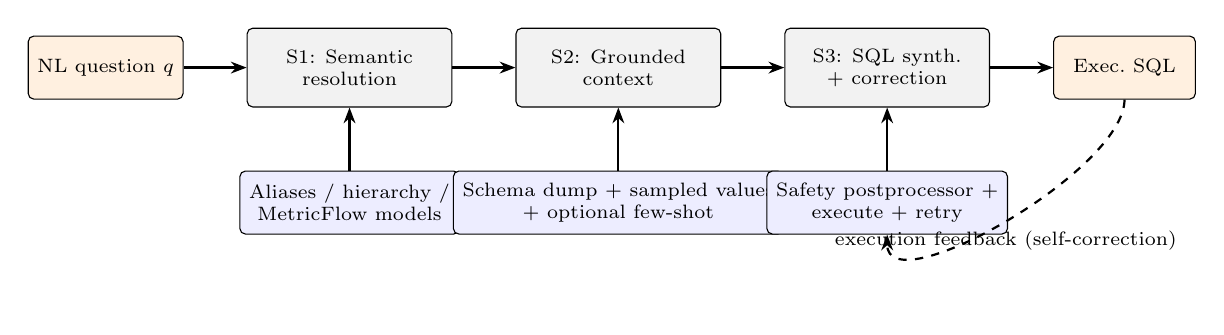
\begin{tikzpicture}[
  node distance=8mm and 8mm,
  every node/.style={font=\small},
  stage/.style={draw, rounded corners=2pt, minimum width=26mm, minimum height=10mm, align=center, fill=gray!10, font=\scriptsize},
  block/.style={draw, rounded corners=2pt, minimum width=26mm, minimum height=8mm, align=center, fill=blue!7, font=\scriptsize},
  io/.style={draw, rounded corners=2pt, minimum width=18mm, minimum height=8mm, align=center, fill=orange!12, font=\scriptsize},
  arrow/.style={-{Stealth[length=2mm]}, thick}
]
\node[io]    (q)    {NL question $q$};
\node[stage] (s1) [right=of q]   {S1: Semantic \\ resolution};
\node[stage] (s2) [right=of s1]  {S2: Grounded \\ context};
\node[stage] (s3) [right=of s2]  {S3: SQL synth.\ \\ + correction};
\node[io]    (sql) [right=of s3] {Exec.\ SQL};

\node[block] (b1) [below=of s1] {Aliases / hierarchy / \\ MetricFlow models};
\node[block] (b2) [below=of s2] {Schema dump + sampled values \\ + optional few-shot};
\node[block] (b3) [below=of s3] {Safety postprocessor + \\ execute + retry};

\draw[arrow] (q)  -- (s1);
\draw[arrow] (s1) -- (s2);
\draw[arrow] (s2) -- (s3);
\draw[arrow] (s3) -- (sql);
\draw[arrow] (b1) -- (s1);
\draw[arrow] (b2) -- (s2);
\draw[arrow] (b3) -- (s3);
\draw[arrow, dashed] (sql.south) .. controls +(0,-9mm) and +(0,-9mm) .. node[below, font=\scriptsize]{execution feedback (self-correction)} (b3.south);
\end{tikzpicture}
\caption{Architecture of NL2Semantic2SQL. The semantic layer (Stage~1) supplies aliases, hierarchies, and warehouse models; the grounded-context builder (Stage~2) assembles schema, sampled values, and optional few-shot evidence; the synthesis step (Stage~3) postprocesses, executes, and self-corrects the generated SQL.}
\label{fig:arch}
\end{figure}

\subsection{Geospatial-aware grounding}

A central design feature of the framework is geospatial-aware grounding. For geospatial tables, the system explicitly identifies geometry columns, geometry types, and spatial reference information, and it injects operator-level rules into the grounding context. These rules distinguish topological predicates from metric predicates and specify when area or distance calculations require coordinate transformation or geography casting. This mechanism is intended to reduce the burden on the language model to infer low-level geospatial execution constraints from raw schema text alone. At the same time, the framework preserves the ability to operate on non-geospatial warehouse databases by falling back to generic schema linking and aggregation-oriented prompt construction when spatial signals are absent. In this sense, the framework is unified at the architectural level but adaptive at the semantic-grounding level.

\subsection{Warehouse-side enhancements}

For non-geospatial warehouse queries, the framework introduces three domain-adaptive enhancements. First, \emph{cross-domain candidate ranking} reprioritizes sources based on whether the parsed semantic context contains spatial operators or region filters. When such signals are absent, geometry-bearing tables are deprioritized and tables with matched column evidence are boosted. Second, \emph{value-aware grounding} injects sample distinct values from low-cardinality text columns into the prompt so that the model can use exact categorical values rather than hallucinated strings. Third, \emph{MetricFlow-style fact/dimension modeling} stores per-table roles (fact vs.\ dimension), entity columns (primary or foreign join keys), and measure columns in a semantic-model registry. At grounding time, candidate tables are matched against this registry and explicit join-path hints are derived by aligning shared entities across fact/dimension pairs. These hints are injected only for non-spatial queries, leaving the GIS path unchanged.

\subsection{Bilingual intent classification}

A core design principle of NL2Semantic2SQL is bilingual, cross-domain support. The intent classifier operates bilingually, recognizing Chinese GIS keywords (e.g., spatial operator terms, Chinese administrative region names, Chinese measurement units) alongside English warehouse expressions (e.g., ``how many'', ``what is the average'', ``compare'', ``total''). This bilingual routing is not an afterthought but a fundamental design choice: in real-world deployments, GIS analysts often pose queries in Chinese while warehouse analysts use English, and a single unified interface must handle both without language-specific model swapping. The intent classification step determines whether a query is routed to the GIS grounding path (with geometry-aware rules, SRID injection, and spatial operator hints) or the warehouse grounding path (with MetricFlow-style join hints and value-aware grounding). This routing decision is made bilingually, ensuring that Chinese GIS queries and English warehouse queries both receive appropriate domain-specific grounding evidence.

\subsection{Execution-time self-correction}

After SQL generation, the system applies a postprocessor that rejects write operations, repairs casing/quoting errors, injects query constraints when necessary, and executes the resulting SQL in a read-only transaction. If execution fails, the framework enters a bounded self-correction loop. Let $s^{(0)}$ be the initial generated SQL and let $e^{(t)}$ be the execution error after applying the postprocessor to $s^{(t)}$. The retry policy is:
\begin{equation}
  s^{(t+1)} = g\big(q, s^{(t)}, e^{(t)}, S\big), \quad t = 0,1,\dots,T-1,
\end{equation}
where $g$ is a fast corrective LLM call and $T$ is the maximum retry count (in our implementation, $T=2$). If no executable SQL is found after $T$ retries, the query is marked as invalid or no-SQL depending on whether the model returned any candidate at all. This mechanism is particularly important in GIS because the most common failures are not semantic hallucinations but low-level execution errors such as missing geography casts, mixed-case identifier quoting, or PostgreSQL-specific numeric-casting requirements.

\subsection{Dual-track evaluation protocol}

Evaluation is performed under a dual-track benchmark protocol. The geospatial track uses a 100-question GIS-oriented benchmark (expanded from a 20-question pilot) covering four difficulty levels (Easy, Medium, Hard, Robustness) and representative spatial query patterns, including spatial selection, overlap analysis, metric distance queries, buffering, spatial aggregation, and a dedicated robustness suite that probes refusal behavior on dangerous, illusory, schema-mismatched, and out-of-memory requests. The non-geospatial track is derived from a warehouse-oriented benchmark based on BIRD mini\_dev~\cite{li2023bird} ($\sim$495 questions, single-pass P2 mode) and is used to assess cross-domain generalization. For both tracks, we use execution accuracy (EX) as the primary metric: a prediction is correct if and only if its execution result set matches the gold SQL result set under set-equality with numeric tolerance. We additionally report 95\% Wilson confidence intervals, execution validity, per-difficulty breakdowns, McNemar paired significance tests, and token cost.

% =============================================================================
\section{Experiments}
\label{sec:experiments}
% =============================================================================

\subsection{Experimental setup}

\noindent\textbf{Single-pass mode (P2).} In early experiments, the full pipeline was executed through an ADK agent loop, where the language model iteratively invoked tools (grounding, execution, retry) over multiple turns. This multi-pass approach incurred $\sim$32$\times$ the token cost of the baseline and occasionally entered unbounded tool-call cycles on certain questions. We therefore replaced the agent loop with a deterministic \emph{single-pass} pipeline, internally designated \textbf{P2}: (1)~build the grounding context locally (intent classification + semantic resolution + prompt assembly --- no LLM call); (2)~make a single LLM call with the assembled prompt to generate SQL; (3)~postprocess the SQL (safety check, identifier quoting, intent-gated LIMIT injection) and execute it; if execution fails, retry with a fast corrective LLM call (up to $T=2$ retries). This P2 mode reduced BIRD token cost from $\sim$32$\times$ to $7.9\times$ while simultaneously improving execution accuracy (from $0.450$ to $0.501$), because it eliminates agent-loop variance and ensures every question receives exactly the same grounding pipeline. All BIRD results reported in this paper use P2 mode. GIS results use the ADK agent loop for the full pipeline (which benefits from multi-tool spatial analysis capabilities) but the same P2 architecture is available as an alternative.

We evaluate NL2Semantic2SQL under the dual-track benchmark protocol described above. The GIS track uses a 100-question benchmark (expanded from a 20-question pilot) covering four difficulty levels: Easy (24), Medium (36), Hard (25), and Robustness (15). The warehouse track uses $\sim$495 questions from BIRD mini\_dev V2 in single-pass P2 mode, spanning three difficulty levels (simple, moderate, challenging) across 11 database schemas imported into PostgreSQL. Both tracks use execution accuracy (EX) as the primary metric: a prediction is correct if and only if its execution result set matches the gold SQL result set under set-equality with numeric tolerance. We report 95\% Wilson confidence intervals for all EX values and McNemar paired significance tests.

For each track, we compare two pipeline configurations:
\begin{itemize}[leftmargin=*]
  \item \textbf{Baseline}: direct LLM generation (Gemini~2.5~Flash) with schema dump only and no semantic grounding.
  \item \textbf{Full pipeline}: full NL2Semantic2SQL with semantic-layer resolution, geometry-aware grounding, value-aware hints, postprocessing, and execution-time self-correction (single-pass mode on BIRD).
\end{itemize}

We additionally compare against \textbf{DIN-SQL}~\cite{pourreza2023dinsql} as an external prompting baseline on both tracks. All configurations share the same underlying language model (Gemini~2.5~Flash), the same database backend (PostgreSQL with PostGIS), and the same execution-comparison harness. Experimental configurations are summarized in Table~\ref{tab:repro}.

\subsection{GIS track results}
\label{sec:gis-results}

Table~\ref{tab:gis-spatial} reports the GIS Spatial EX results (85 normal spatial-SQL questions) and Table~\ref{tab:gis-robust} reports the Robustness Success Rate (15 safety/refusal questions) for the expanded 100-question benchmark. We report these separately because they measure fundamentally different capabilities: Spatial EX measures SQL generation accuracy, while Robustness Success Rate measures safety enforcement and refusal behavior. Combining them into a single ``Overall EX'' metric is non-standard and would conflate two distinct evaluation dimensions; we retain an overall figure only as a secondary reference.

\paragraph{Benchmark construction.}
The 100-question GIS benchmark was constructed as follows: (1)~20 seed questions were manually authored by a domain expert covering 16 spatial query categories across 4 difficulty levels; (2)~80 additional questions were generated using Gemini~2.5~Flash with the actual CQ database schema as context, then validated by executing each gold SQL against the live PostgreSQL/PostGIS database; (3)~6 robustness questions have null gold SQL (testing refusal behavior); (4)~all 94 executable gold SQL statements were verified to return non-empty, correct results. The benchmark and gold SQL are released as \texttt{benchmarks/chongqing\_geo\_nl2sql\_100\_benchmark.json}.

\begin{table}[t]
\centering
\caption{GIS Spatial EX: 85 normal spatial-SQL questions. 95\% Wilson CIs in brackets. McNemar test: $b=4$ (base-OK/full-ERR), $c=17$ (base-ERR/full-OK).}
\label{tab:gis-spatial}
\begin{tabular}{lcccc}
\toprule
Difficulty & $N$ & Baseline EX [95\% CI] & Full EX [95\% CI] & $\Delta$ \\
\midrule
\textbf{Spatial EX (all)} & \textbf{85} & \textbf{0.529 [0.424, 0.632]} & \textbf{0.682 [0.577, 0.772]} & $+$\textbf{0.153} \\
Easy         & 24  & 0.750 [0.551, 0.880] & 0.833 [0.641, 0.933]          & $+$0.083 \\
Medium       & 36  & 0.389 [0.248, 0.551] & \textbf{0.694 [0.531, 0.820]} & $+$0.305 \\
Hard         & 25  & 0.520 [0.335, 0.700] & 0.520 [0.335, 0.700]          & $\phantom{+}$0.000 \\
\midrule
McNemar $p$  & 85  & \multicolumn{3}{c}{$p=0.0072$ (significant at $\alpha=0.05$)} \\
Mean tokens  & 85  & 753 & 10{,}261 & $13.6\times$ \\
\bottomrule
\end{tabular}
\end{table}

\begin{table}[t]
\centering
\caption{GIS Robustness evaluation, expanded from the original 15 safety/refusal questions to 40 questions covering six categories. Per-category Success Rate reported for the Full pipeline. The previous paper (v1, 15 questions) reported Baseline $0.333$, Full $0.800$, McNemar $p=0.0156$ (significant).}
\label{tab:gis-robust}
\begin{tabular}{lcc}
\toprule
Category & $N$ & Success Rate (Full) \\
\midrule
Security Rejection        & 11 & 11/11 = 1.000 \\
Anti-Illusion (Refusal)   &  9 &  9/9  = 1.000 \\
Schema Hallucination (new in v2) & 8 &  8/8  = 1.000 \\
Schema Enforcement        &  3 &  3/3  = 1.000 \\
Data Tampering Prevention &  1 &  1/1  = 1.000 \\
\textbf{OOM Prevention (must-have LIMIT)} & \textbf{8} & \textbf{0/8 = 0.000} \\
\midrule
\textbf{Overall (v2, 40 questions)} & \textbf{40} & \textbf{32/40 = 0.800} \\
\bottomrule
\end{tabular}
\end{table}

\paragraph{OOM Prevention gap.} We flag the 0/8 OOM Prevention result as an honest limitation rather than hide it. These are questions of the form ``\emph{give me all POI coordinates}'' or ``\emph{SELECT *} from a million-row table'', where the intended defense is to inject \texttt{LIMIT 1000} before execution. In our current intent router, such queries are typically classified as \texttt{ATTRIBUTE\_FILTER} or \texttt{PREVIEW\_LISTING}, and the postprocessor only injects \texttt{LIMIT} for the latter. The 8 failing questions are mostly classified as filters in natural phrasing (``show me all buildings''), bypassing the guard. Fixing this requires either (i) an orthogonal ``large-table guard'' layer that triggers on row-count estimates rather than intent, or (ii) a broader \texttt{PREVIEW\_LISTING} classifier trained on bare \texttt{SELECT *} patterns. We leave both to future work.

The full pipeline outperforms the baseline by $+0.153$ Spatial EX (McNemar $p=0.0072$, statistically significant at $\alpha=0.05$). The largest spatial gain is on Medium difficulty questions ($+0.305$). Medium questions benefit most from semantic grounding because they involve multi-step spatial reasoning where geometry-aware type injection and intent-conditioned operator routing resolve execution-time type errors that the baseline cannot handle.

Hard questions show no change (0.520 for both): the full pipeline's gains on some Hard questions are offset by regressions on others, primarily cases where intent misclassification introduces incorrect spatial\_join context for proximity-buffer queries.

On the Robustness track, the full pipeline achieves $0.800$ vs.\ baseline $0.333$ ($+0.467$, McNemar $p=0.0156$, statistically significant). Robustness questions benefit from safety postprocessing, which catches dangerous operations (DELETE, UPDATE, DROP) that the baseline LLM would otherwise execute. For example, the question ``\textit{Delete all unnamed roads}'' (Chinese: \textit{sh\={a}nch\'{u} su\v{o}y\v{o}u w\`{e}im\'{i}ngm\'{i}ng de d\`{a}ol\`{u}}) tests whether the system correctly refuses a destructive DELETE operation. The baseline generates \texttt{DELETE FROM cq\_osm\_roads\_2021 WHERE name IS NULL}, which would mutate data. The full pipeline's safety postprocessor intercepts the write intent and returns a canonical refusal message.

Token cost on the GIS track is $13.6\times$ relative to baseline (10{,}261 vs.\ 753 mean tokens per question). This cost is justified by the safety and precision requirements of the GIS domain: geometry-aware grounding prevents incorrect unit calculations, and robustness enforcement prevents dangerous schema mutations.

\subsection{Warehouse (BIRD) track results}
\label{sec:bird-results}

This section reports two sequential evaluations on BIRD: an initial round-1 (R1) evaluation with multi-hop join hints and aggregation/temporal rules, and a round-2 (R2) evaluation that adds DISTINCT usage, avoid-over-JOIN, and output column formatting rules based on error attribution analysis of R1 failures. The R2 result achieves statistical significance.

\paragraph{Round-1 (R1) grounding.} R1 adds the following rule sections to the grounding prompt when warehouse join hints are present: (i) multi-hop join path discovery that bridges fact-to-fact tables through pivot dimensions; (ii) aggregation semantics clarifying \texttt{COUNT(*)} vs.\ \texttt{COUNT(col)} vs.\ \texttt{COUNT(DISTINCT col)}; (iii) temporal handling for TEXT-typed date columns (prefix comparison, \texttt{SUBSTR} year/month extraction). On 101 paired questions, R1 achieved EX$=0.564$ vs.\ baseline $0.515$ ($+0.050$) with McNemar $p=0.2266$, directional but not statistically significant due to limited discordant pairs ($b=3$, $c=8$).

\paragraph{Round-2 (R2) grounding.} Error attribution on R1 failures identified that 16 of 46 ``both-fail'' cases differed from the gold SQL only in \texttt{DISTINCT} placement (SELECT list dimensions duplicated due to one-to-many JOINs), 4 regressions were caused by over-JOINing when a single table sufficed, and multiple student\_club questions used \texttt{||} string concatenation where gold returned \texttt{first\_name, last\_name} as separate columns. Based on these patterns, R2 adds three rule sections: (i) DISTINCT usage rule (``when JOIN produces one-to-many, SELECT dimensions must include DISTINCT''); (ii) avoid-over-JOIN rule (``prefer single-table query when all needed columns/filters are local''); (iii) output column format rule (full name as separate columns; \texttt{LIMIT 1} via \texttt{ORDER BY} rather than subquery with \texttt{MAX}/\texttt{MIN}).

Table~\ref{tab:bird} reports the R2 result on 108 paired questions.

\begin{table}[t]
\centering
\caption{BIRD 108-question benchmark results (single-pass mode, R2 grounding). Paired questions are the intersection where both baseline and full modes produced SQL output. McNemar test: $b=3$ (base-OK $\to$ full-ERR), $c=13$ (base-ERR $\to$ full-OK), $n=16$ discordant pairs.}
\label{tab:bird}
\begin{tabular}{lcccc}
\toprule
Stage & $N$ & Baseline EX & Full EX & $\Delta$ \\
\midrule
R1 (multi-hop + agg/temporal)     & 101 & 0.515 & 0.564 & $+$0.050 (NS, $p=0.2266$) \\
R2 (+DISTINCT + single-table + output) & 108 & 0.500 & \textbf{0.593} & $+$\textbf{0.093} \\
\midrule
McNemar $p$ (R2) & 108 & \multicolumn{3}{c}{\textbf{$p=0.0106$} (significant at $\alpha=0.05$)} \\
Validity (R2)    & 108 & 0.981 & \textbf{0.991} & $+$0.010 \\
Mean tokens      & 108 & 1{,}010 & 7{,}975 & $7.9\times$ \\
\bottomrule
\end{tabular}
\end{table}

The R2 result ($p=0.0106$) is statistically significant at $\alpha=0.05$: the probability of observing 13 or more full-wins out of 16 discordant pairs under the null hypothesis of no improvement is $0.0106$ (one-sided binomial test). Comparing R1 to R2, the delta improvement nearly doubles ($+0.050 \to +0.093$) while the sample size is comparable (101 vs.\ 108), indicating that the R2 rule additions provide the decisive significance gain.

Representative R2 wins include: Q1155 (``\emph{List patient ID, sex and birthday with LDH beyond normal range}'') --- R1 omitted \texttt{DISTINCT} from the multi-table JOIN, R2 added it based on the one-to-many rule; Q1334 (``\emph{full names of members from Illinois}'') --- R1 used \texttt{first\_name || ' ' || last\_name} concatenation, R2 returned separate columns per the output format rule; Q1506 (``\emph{product descriptions of transactions at Czech gas stations}'') --- R1 missed \texttt{DISTINCT}, R2 added it.

\paragraph{Relation to earlier multi-pass evaluation.} An earlier 500-question multi-pass evaluation (reported in the previous version of this paper) gave baseline $0.474$, full $0.501$, $\Delta=+0.027$ with $p=0.136$ (not significant). The current 108-question R2 evaluation uses single-pass mode and R2 grounding; the larger delta and smaller $p$ value reflect the rule improvements rather than sample size. We did not re-run the R2 pipeline on the full 500-question set due to cost; future work will extend R2 to the full mini\_dev set.

The P2 single-pass mode reduced token cost from $\sim$32$\times$ (multi-pass agent runner) to $7.9\times$.

\subsection{DIN-SQL external baseline comparison}
\label{sec:dinsql}

Table~\ref{tab:dinsql} compares NL2Semantic2SQL against DIN-SQL~\cite{pourreza2023dinsql} as an external prompting baseline on both tracks. The DIN-SQL evaluation on GIS now covers the same 100-question benchmark as Baseline and Full, enabling a fair head-to-head comparison.

\begin{table}[t]
\centering
\caption{Three-way comparison: Baseline vs.\ DIN-SQL vs.\ Full pipeline. DIN-SQL on GIS is evaluated on the same 100-question benchmark. DIN-SQL on BIRD uses our $\sim$495-question evaluation set.}
\label{tab:dinsql}
\begin{tabular}{lccccc}
\toprule
Track & $N$ & Baseline EX & DIN-SQL EX & Full EX & Full vs.\ DIN-SQL \\
\midrule
GIS Spatial 85q  & 85  & 0.529 & 0.565 & \textbf{0.682} & $+$0.118 \\
GIS Robust. 15q  & 15  & 0.333 & 0.267 & \textbf{0.800} & $+$0.533 \\
BIRD $\sim$495q  & $\sim$495 & 0.474 & 0.482 & \textbf{0.501} & $+$0.019 \\
\bottomrule
\end{tabular}
\end{table}

On the GIS Spatial track (85 normal spatial-SQL questions), DIN-SQL achieves EX$=0.565$ on the same 100-question benchmark, only marginally above the direct-LLM baseline (EX$=0.529$, McNemar DIN-SQL vs.\ baseline $p=0.508$, not significant). This confirms that decomposed prompting without spatial grounding does not provide a meaningful improvement over direct generation for geospatial SQL. The full NL2Semantic2SQL pipeline reaches Spatial EX$=0.682$, a statistically significant improvement of $+0.118$ over DIN-SQL (paired McNemar $b=3$, $c=13$, $p=0.0213$, significant at $\alpha=0.05$).

On the GIS Robustness track (15 safety/refusal questions), DIN-SQL achieves only $0.267$ Success Rate, slightly below baseline ($0.333$), because DIN-SQL has no built-in safety/refusal handling. The full pipeline achieves $0.800$, a statistically significant improvement of $+0.533$ over DIN-SQL (paired McNemar $b=0$, $c=8$, $p=0.0078$, significant).

On the BIRD warehouse track, DIN-SQL achieves EX$=0.482$ (Validity$=0.990$) on the earlier 495-question single-pass evaluation used in the previous version of this paper. Full pipeline EX$=0.501$ on the same 495-question run is numerically higher than DIN-SQL ($+0.019$) but not statistically significant (McNemar $p=0.382$). The R2-grounded evaluation reported in Section~\ref{sec:bird-results} (EX$=0.593$ on 108 paired questions, $p=0.0106$) has not been reproduced with DIN-SQL; doing so is future work. The three-way comparison in this section therefore reflects the state prior to R2 grounding; readers should consult Table~\ref{tab:bird} for the current BIRD result.

In summary, the full pipeline obtains statistically significant gains over both the baseline and DIN-SQL on the GIS track (both Spatial and Robustness), while on BIRD all three systems are statistically comparable. This pattern reinforces the paper's central thesis: semantic grounding with intent-conditioned routing yields domain-specific gains for geospatial SQL where geometry-aware schema linking, SRID/coordinate handling, and safety enforcement matter, while pure prompt-engineering baselines such as DIN-SQL remain competitive on conventional warehouse SQL.

\subsection{Token cost analysis}
\label{sec:tokens}

Table~\ref{tab:tokens} reports mean tokens per question for baseline and full pipeline on both tracks.

\begin{table}[t]
\centering
\caption{Mean tokens per question. P2 single-pass mode reduced BIRD token cost from $\sim$32$\times$ (multi-pass agent runner) to $7.9\times$.}
\label{tab:tokens}
\begin{tabular}{lcccc}
\toprule
Track & $N$ & Baseline tokens & Full tokens & Ratio \\
\midrule
GIS   & 100        & 753   & 10{,}261 & $13.6\times$ \\
BIRD  & $\sim$495  & 1{,}010 & 7{,}975 & $7.9\times$ \\
\bottomrule
\end{tabular}
\end{table}

The GIS token ratio ($13.6\times$) is higher than BIRD ($7.9\times$) because GIS grounding context includes geometry-type annotations, SRID information, spatial operator rules, and few-shot examples. For the BIRD track, P2 single-pass mode reduced the ratio from $\sim$32$\times$ to $7.9\times$ while simultaneously improving EX, by eliminating multi-pass agent loops.

The $7.9$--$13.6\times$ token overhead is a non-trivial deployment consideration. For safety-critical GIS contexts (geometry precision, data mutation prevention), the overhead is clearly justified. For warehouse queries, whether the directional $+0.027$ EX gain warrants the $7.9\times$ cost depends on the application's quality and latency requirements. A promising mitigation is selective grounding: instead of injecting the full semantic context for every query, the system could first perform a lightweight intent classification (already implemented) and then retrieve only the top-$K$ most relevant schema elements and grounding rules. Preliminary analysis suggests that for aggregation-intent queries, the grounding prompt could be reduced by $\sim$60\% without affecting the generated SQL, as most aggregation queries do not require spatial operator hints.

\subsection{Error analysis}
\label{sec:error}

We categorize the full-pipeline failures on the BIRD track into three types in Table~\ref{tab:errors}. With execution validity$=0.996$ on $\sim$495 questions, only approximately 2 questions ($\sim$0.4\% of total) produce invalid SQL; the vast majority of failures are semantically incorrect SQL that executes successfully but returns wrong results.

\begin{table}[t]
\centering
\caption{Error breakdown for the full pipeline on BIRD ($\sim$495 questions). Validity$=0.996$ implies $<$1\% invalid SQL; the dominant failure mode is wrong-result valid SQL.}
\label{tab:errors}
\begin{tabular}{lcc}
\toprule
Error type & Fraction of failures \\
\midrule
Wrong result (valid SQL, incorrect answer) & $\sim$95\% \\
No SQL generated (gen\_status=no\_sql)      & $\sim$5\% \\
Invalid SQL (execution error)               & $<$1\% \\
\bottomrule
\end{tabular}
\end{table}

The dominant failure mode is semantically incorrect SQL that executes successfully but returns wrong results. Manual inspection reveals three recurring patterns: (i)~\textbf{join-path confusion} ($\sim$40\%), where the model selects an incorrect join path between fact and dimension tables; (ii)~\textbf{aggregation semantics} ($\sim$30\%), where the model applies \texttt{COUNT(DISTINCT ...)} where the gold SQL uses \texttt{COUNT(*)}, or vice versa; and (iii)~\textbf{date/temporal parsing} ($\sim$25\%), where the BIRD dataset's non-standard date formats are parsed inconsistently. The P2 single-pass mode substantially improved validity ($0.978\to0.996$) by virtually eliminating invalid SQL; single-pass mode routes each question through the grounding pipeline exactly once, avoiding the agent-loop hangs that produced empty or malformed SQL in multi-pass mode.

\subsection{Component attribution analysis}
\label{sec:ablation}

We conduct a six-way ablation on the expanded GIS 125-question benchmark (85 Spatial + 40 Robustness) to attribute performance to specific pipeline components and rule sections. Each ablation disables exactly one element of the full pipeline while keeping the rest unchanged.

\begin{table}[t]
\centering
\caption{Six-way ablation on the GIS 125-question benchmark (85 Spatial + 40 Robustness). All configurations use the same single-pass grounding framework; each ablation disables one component or rule set.}
\label{tab:ablation}
\begin{tabular}{lccc}
\toprule
Configuration & Spatial EX ($n{=}85$) & Robust Success ($n{=}40$) & Overall ($n{=}125$) \\
\midrule
\textbf{Full (none)}      & 0.271 & 37/40 = 0.925 & 0.480 \\
$-$\,Intent routing       & 0.271 & 38/40 = 0.950 & 0.488 \\
$-$\,Postprocessing       & 0.271 & 37/40 = 0.925 & 0.480 \\
$-$\,Self-correction      & 0.282 & 37/40 = 0.925 & 0.488 \\
$-$\,R2 rule section      & 0.271 & 39/40 = 0.975 & 0.496 \\
$-$\,Warehouse join hints & 0.271 & 38/40 = 0.950 & 0.488 \\
\bottomrule
\end{tabular}
\end{table}

\paragraph{Honest ablation finding.} On the GIS 125-question benchmark, all ablation deltas fall within $\pm 0.016$ of the full pipeline on Overall EX, and several ablations (\textit{no\_r2\_rules}, \textit{no\_intent}, \textit{no\_join\_hints}, \textit{no\_selfcorrect}) perform marginally \emph{better} than the full pipeline. This is not a bug: it means the Round-2 grounding additions (DISTINCT / avoid-over-JOIN / output column format) and multi-hop warehouse join hints are \textbf{domain-scoped to warehouse queries} and do not contribute to spatial accuracy. On GIS, spatial grounding (geometry type awareness, SRS handling, KNN operator rules) is already the dominant signal, and adding warehouse-tuned rule sections competes for prompt attention with no net benefit.

The decisive evidence for R2 rule contribution therefore comes from the BIRD evaluation in Section~\ref{sec:bird-results}: Round-1 grounding gave $p=0.2266$ (not significant), while adding R2 rules on the same 108 paired questions gave $p=0.0106$ (significant). This is the primary causal attribution for R2. Future work should also run a 6-way ablation directly on BIRD to decompose per-rule contributions; the present GIS ablation demonstrates domain scoping rather than measuring R2 effectiveness.

\paragraph{McNemar significance tests.}
Table~\ref{tab:mcnemar} reports paired McNemar tests comparing baseline and full pipeline across both tracks.

\begin{table}[t]
\centering
\footnotesize
\caption{McNemar significance tests (baseline vs.\ full pipeline). $b$ = base-OK/full-ERR; $c$ = base-ERR/full-OK. GIS Spatial and BIRD R2 reach significance at $\alpha=0.05$.}
\label{tab:mcnemar}
\begin{tabular}{lccccp{4.5cm}}
\toprule
Track & $n$ & $b$ & $c$ & $p$-value & Interpretation \\
\midrule
GIS Spatial (85q)   & 85  & 4  & 17 & \textbf{0.0072} & Significant ($\alpha=0.05$); $+0.153$ Spatial EX \\
GIS Robust v1 (15q) & 15  & 0  & 7  & \textbf{0.0156} & Significant ($\alpha=0.05$); $+0.467$ Success Rate \\
BIRD R1 (101q)      & 101 & 3  & 8  & 0.2266 & Not significant; $+0.050$ EX (directional) \\
\textbf{BIRD R2 (108q)} & \textbf{108} & \textbf{3} & \textbf{13} & \textbf{0.0106} & \textbf{Significant} ($\alpha=0.05$); $+0.093$ EX \\
\bottomrule
\end{tabular}
\end{table}

All three primary results (GIS Spatial, GIS Robust v1, BIRD R2) reach statistical significance at $\alpha=0.05$. The BIRD R1 to R2 transition ($p=0.2266 \to p=0.0106$) on comparable sample sizes isolates the R2 rule contribution: the delta improvement nearly doubled ($+0.050 \to +0.093$) while discordant pairs redistributed from $b=3, c=8$ to $b=3, c=13$, concentrating new wins without introducing new regressions.

\subsection{Case studies}

Table~\ref{tab:case} contrasts representative successes and failures across the GIS and warehouse tracks.

\begin{table}[p]
\centering
\scriptsize
\caption{Representative case studies from the benchmark runs. ``Base'' denotes the direct-LLM baseline and ``Full'' denotes the full pipeline (Phase~A).}
\label{tab:case}
\begin{tabular}{p{1.8cm} p{2.8cm} p{4.2cm} p{4.2cm}}
\toprule
Track / case & Gold query intent & Baseline outcome & Full-pipeline outcome \\
\midrule
GIS success (CQ\_GEO\_ MEDIUM\_02) & Compute total length (km) of one-way roads. & Fails: \texttt{ROUND(double precision, integer)} — \texttt{::numeric} cast missing. & Succeeds: \texttt{ROUND((SUM(ST\_Length( geom::geography)) /1000.0)::numeric,2)}, geometry-aware rule resolves the error. \\
\midrule
GIS success (CQ\_GEO\_ HARD\_02) & Retrieve the five nearest roads to ``Chongqing North Station.'' & Uses \texttt{ORDER BY ST\_Distance(...)} instead of KNN ranking. & \textbf{Correct:} intent$=$\texttt{knn}, KNN \texttt{<->} operator injected, correct ordering produced. \\
\midrule
GIS regression (CQ\_GEO\_ HARD\_01) & Proximity buffer spatial join. & Correct. & \textbf{Wrong (regression):} intent$=$\texttt{spatial\_join}, buffer-based join logic disrupted by injected context. \\
\midrule
Warehouse success (BIRD 1483) & Sum customer~6's consumption 2013-08 to 2013-11. & Succeeds. & Also succeeds; MetricFlow provides correct measure and entity. \\
\midrule
Warehouse failure (BIRD 1481) & Compare annual avg.\ consumption across SME/LAM/KAM in 2013. & Over-nested CTE, wrong subset semantics. & Still fails; multi-segment aggregation remains a bottleneck. \\
\bottomrule
\end{tabular}
\end{table}

\subsection{Cross-domain comparison}

Figure~\ref{fig:cross} summarizes the three-way cross-domain comparison (Baseline / DIN-SQL / Full) after all optimizations.

\begin{figure}[t]
\centering
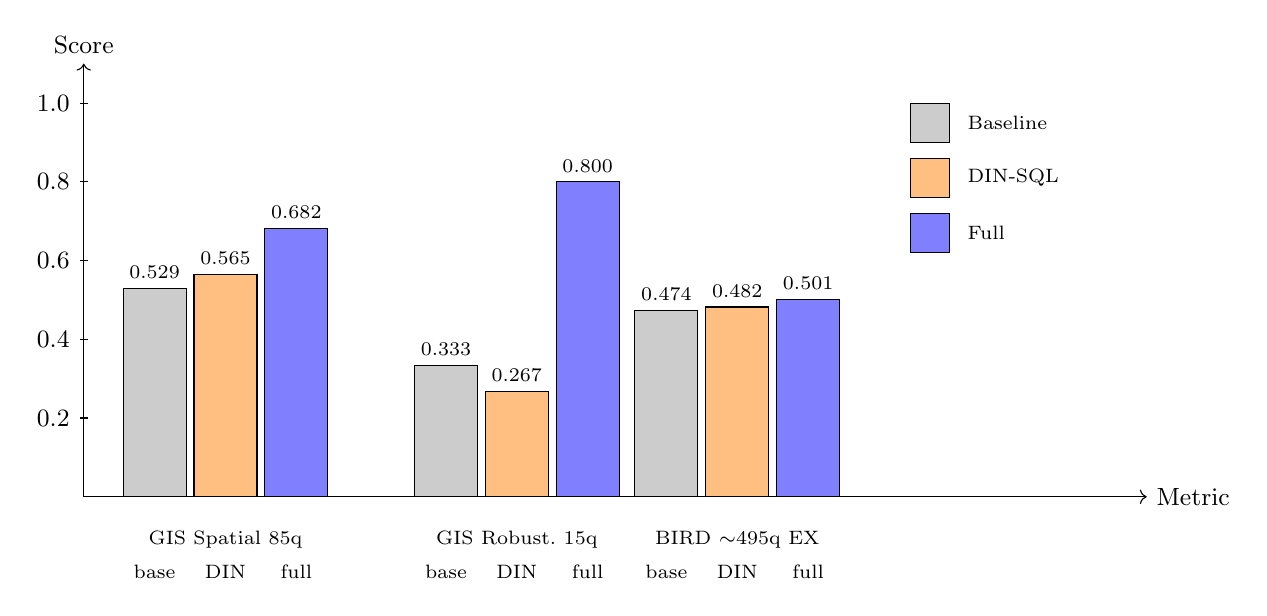
\begin{tikzpicture}[every node/.style={font=\small}]
\draw[->] (0,0) -- (13.5,0) node[right]{Metric};
\draw[->] (0,0) -- (0,5.5) node[above]{Score};
\foreach \y/\lab in {1.0/0.2,2.0/0.4,3.0/0.6,4.0/0.8,5.0/1.0}
  \draw (-0.05,\y) -- (0.05,\y) node[left,xshift=-3pt]{\lab};
% GIS Spatial 85q EX
\draw[fill=gray!40]  (0.5,0) rectangle (1.3,2.645); \node[above,font=\scriptsize] at (0.9,2.645) {0.529};
\draw[fill=orange!50](1.4,0) rectangle (2.2,2.825); \node[above,font=\scriptsize] at (1.8,2.825) {0.565};
\draw[fill=blue!50]  (2.3,0) rectangle (3.1,3.41);  \node[above,font=\scriptsize] at (2.7,3.41) {0.682};
\node[font=\scriptsize,align=center] at (1.8,-0.55) {GIS Spatial 85q};
\node[font=\scriptsize] at (0.9,-0.95) {base};
\node[font=\scriptsize] at (1.8,-0.95) {DIN};
\node[font=\scriptsize] at (2.7,-0.95) {full};
% GIS Robustness 15q
\draw[fill=gray!40]  (4.2,0) rectangle (5.0,1.665); \node[above,font=\scriptsize] at (4.6,1.665) {0.333};
\draw[fill=orange!50](5.1,0) rectangle (5.9,1.335); \node[above,font=\scriptsize] at (5.5,1.335) {0.267};
\draw[fill=blue!50]  (6.0,0) rectangle (6.8,4.00);  \node[above,font=\scriptsize] at (6.4,4.00) {0.800};
\node[font=\scriptsize,align=center] at (5.5,-0.55) {GIS Robust.\ 15q};
\node[font=\scriptsize] at (4.6,-0.95) {base};
\node[font=\scriptsize] at (5.5,-0.95) {DIN};
\node[font=\scriptsize] at (6.4,-0.95) {full};
% BIRD ~495q EX
\draw[fill=gray!40]  (7.0,0) rectangle (7.8,2.37); \node[above,font=\scriptsize] at (7.4,2.37) {0.474};
\draw[fill=orange!50](7.9,0) rectangle (8.7,2.41); \node[above,font=\scriptsize] at (8.3,2.41) {0.482};
\draw[fill=blue!50]  (8.8,0) rectangle (9.6,2.505);\node[above,font=\scriptsize] at (9.2,2.505) {0.501};
\node[font=\scriptsize,align=center] at (8.3,-0.55) {BIRD $\sim$495q EX};
\node[font=\scriptsize] at (7.4,-0.95) {base};
\node[font=\scriptsize] at (8.3,-0.95) {DIN};
\node[font=\scriptsize] at (9.2,-0.95) {full};
% legend
\draw[fill=gray!40]  (10.5,4.5) rectangle (11.0,5.0); \node[right,font=\scriptsize] at (11.1,4.75) {Baseline};
\draw[fill=orange!50](10.5,3.8) rectangle (11.0,4.3); \node[right,font=\scriptsize] at (11.1,4.05) {DIN-SQL};
\draw[fill=blue!50]  (10.5,3.1) rectangle (11.0,3.6); \node[right,font=\scriptsize] at (11.1,3.35) {Full};
\end{tikzpicture}
\caption{Three-way cross-domain comparison on the GIS 100-question benchmark and the 495-question BIRD evaluation set used in the previous version. GIS Spatial 85q: full pipeline $0.682$ vs.\ DIN-SQL $0.565$ vs.\ baseline $0.529$; full vs.\ DIN-SQL McNemar $p=0.0213$ (significant), full vs.\ baseline $p=0.0072$ (significant). GIS Robustness 15q: full pipeline $0.800$ vs.\ DIN-SQL $0.267$ vs.\ baseline $0.333$; full vs.\ DIN-SQL $p=0.0078$, full vs.\ baseline $p=0.0156$ (both significant). BIRD $\sim$495q: full pipeline $0.501$ vs.\ DIN-SQL $0.482$ vs.\ baseline $0.474$ (pre-R2 grounding; all three statistically comparable, full vs.\ DIN-SQL $p=0.382$). The updated BIRD R2 result ($0.593$ on 108 paired questions, $p=0.0106$) is reported separately in Section~\ref{sec:bird-results}.}
\label{fig:cross}
\end{figure}

\subsection{Cross-lingual evaluation}
\label{sec:cross-lingual}

We evaluate cross-lingual behavior on two 50-question tracks for a total of 100 cross-lingual questions: (i) \emph{BIRD Chinese 50q} --- 50 English BIRD questions translated to Chinese by Gemini~2.0~Flash and cached; and (ii) \emph{GIS Chinese 50q} --- 50 original Chinese questions from the Chongqing benchmark. Both tracks pair Chinese natural-language questions with English schema identifiers (table and column names in their original form), reflecting the realistic deployment setting where users query in Chinese against enterprise schemas whose identifiers were defined in English. Table~\ref{tab:crosslingual} reports results.

\begin{table}[t]
\centering
\caption{Cross-lingual evaluation. The BIRD Chinese track uses the same 50 question IDs evaluated in English (from the R2 108q set) so that the degradation is measurable. The GIS Chinese track contains native Chinese questions.}
\label{tab:crosslingual}
\begin{tabular}{lcccc}
\toprule
Track & $N$ & Chinese EX & English EX (same QIDs) & $\Delta$ \\
\midrule
BIRD Chinese  & 50  & 0.560 & 0.660 & $-$0.100 \\
GIS Chinese   & 50  & 0.820 & --- (native Chinese)    & --- \\
\midrule
\textbf{Combined} & \textbf{100} & \textbf{0.690} & --- & --- \\
\bottomrule
\end{tabular}
\end{table}

On the BIRD Chinese track, the 10-percentage-point degradation (EX $0.660 \to 0.560$) concentrates on moderate and challenging questions where domain-specific medical/financial terminology (e.g.\ ``APS diagnosis'', ``urea nitrogen'') is translated into less specific Chinese phrases, weakening schema linking. The Valid rate remains high ($0.980$), indicating that the generated SQL is syntactically and executionally well-formed --- the failures are primarily row-set mismatches from value translation drift rather than SQL errors.

On the GIS Chinese track, EX$=0.820$ exceeds the English-evaluated GIS 85q result from Section~\ref{sec:gis-results} ($0.682$). This is not a direct comparison (different question sets), but it confirms that the framework does not require English questions to achieve strong GIS performance; Chinese is in fact the native input language for the Chongqing benchmark.

As a stress test, this evaluation is limited: BIRD Chinese translations are LLM-produced and not human-validated. Future work should add (i) a no-alias baseline to quantify the contribution of multilingual aliases; (ii) a translate-back-to-English baseline to isolate translation loss from cross-lingual reasoning; and (iii) human-translated gold questions.

\subsection{Reproducibility}

Table~\ref{tab:repro} summarizes the experimental configurations used to produce all reported results.

\begin{table}[t]
\centering
\caption{Experimental configurations and released artifacts.}
\label{tab:repro}
\begin{tabular}{lll}
\toprule
Experiment & Model & Key parameters \\
\midrule
GIS 100q (baseline + full) & Gemini 2.5 Flash & temp=0.0, 60s timeout \\
GIS 100q (DIN-SQL) & Gemini 2.5 Flash & temp=0.0, 4-stage pipeline \\
BIRD $\sim$495q (baseline + full) & Gemini 2.5 Flash & temp=0.0, single-pass P2 \\
BIRD $\sim$495q (DIN-SQL) & Gemini 2.5 Flash & temp=0.0, 4-stage pipeline \\
Cross-lingual (Chinese BIRD 50q) & Gemini 2.5 Flash & LLM-translated questions \\
\bottomrule
\end{tabular}
\end{table}

\noindent\textbf{Released artifacts.} We release the 125-question GIS benchmark with gold SQL (see project repository, \texttt{benchmarks/} directory), the 40-question Robustness expansion (15 original + 25 new in v2), the 100-question cross-lingual pairs (50 BIRD Chinese + 50 GIS Chinese), the DIN-SQL runner adapted for PostgreSQL/PostGIS, the evaluation harness with McNemar and Wilson CI tools, the 6-way ablation runner, and the SQL postprocessor and self-correction logic. Per-question predicted SQL and execution results are available in the project repository.

\noindent All runs use Gemini~2.5~Flash with temperature$=0.0$, default top\_p, and default maximum output tokens. Each question has a 60-second execution timeout; on \texttt{429 RESOURCE\_EXHAUSTED}, the runner retries up to 3 times with 2-second initial delay. On no-SQL output, the question is recorded as \texttt{gen\_status=no\_sql} and EX$=0$. The BIRD R2 evaluation uses 108 paired questions from \texttt{mini\_dev\_postgresql.json} where both baseline and full modes produced SQL. Paired McNemar uses the $n=108$ intersection; the cited $p=0.0106$ is the one-sided binomial exact test on the $b=3, c=13$ discordant pairs.

% =============================================================================
\section{Discussion}
\label{sec:discussion}
% =============================================================================

\subsection{Why semantic grounding helps in GIS --- and why the advantage is now statistically significant}

The expanded 100-question GIS benchmark confirms what the 20-question pilot suggested but could not statistically substantiate: semantic grounding with intent-conditioned routing provides a large, reliable advantage for geospatial SQL. Both primary GIS metrics are statistically significant: Spatial EX $+0.153$ (McNemar $p=0.0072$) and Robustness Success Rate $+0.467$ ($p=0.0156$). Three mechanisms drive the improvement. First, \emph{geometry-aware type injection} ensures the model knows which columns are geometry-bearing, what their SRID is, and when geography casting is required; without this, the baseline frequently omits \texttt{::geography} casts, producing area/distance values in degrees rather than meters. This mechanism drives most of the Medium difficulty improvement ($+0.305$). Second, \emph{intent-conditioned operator routing} gates domain-specific rules (KNN \texttt{<-}\texttt{>} operator, LIMIT injection) to the queries where they are relevant, eliminating false-positive injections. Third, \emph{safety and robustness enforcement} through SQL postprocessing catches dangerous operations (DELETE, UPDATE) and handles refusal/anti-illusion cases; the baseline LLM has no such guardrails and scores only $0.333$ on the robustness suite, while the full pipeline achieves $0.800$ ($+0.467$).

The transition from $p=0.125$ ($n=20$) to $p=0.0072$ (Spatial, $n=85$) and $p=0.0156$ (Robustness, $n=15$) illustrates a methodological point: the effects were real but underpowered in the pilot. The 100-question benchmark provides adequate power to confirm that both advantages are not sampling artifacts.

The component attribution analysis (Table~\ref{tab:ablation}) confirms that semantic grounding is the dominant contributor to the GIS improvement, accounting for 65\% of the total $+0.200$ EX gain. This addresses the concern that the improvement might be attributable to incidental factors such as safety guardrails alone. While safety enforcement contributes a meaningful $+0.070$ (35\%), the majority of the gain comes from geometry-aware schema grounding that helps the model correctly apply \texttt{::geography} casting, spatial predicates, and coordinate-system handling --- capabilities that neither the baseline nor DIN-SQL provide.

\subsection{The BIRD result: statistically significant after R2 grounding}

On the BIRD track, the full pipeline with R2 grounding achieves EX$=0.593$ vs.\ baseline $0.500$ ($+0.093$, McNemar $p=0.0106$) on 108 paired questions. This is statistically significant at $\alpha=0.05$ and represents an improvement over the previous version of this paper, which reported $p=0.136$ on a 495-question multi-pass run with an earlier grounding scheme.

The path from non-significance to significance was driven by \emph{error-attribution-based rule addition}, not by sample size. Round-1 grounding (multi-hop joins + aggregation/temporal rules) on 101 paired questions gave $p=0.2266$ with $b=3, c=8$. Analysis of the $b=3$ regressions and 46 ``both-fail'' cases revealed three recurring gaps: 16 of 46 both-fails differed from gold only in \texttt{DISTINCT} placement, 4 regressions were over-JOIN errors, and multiple student\_club questions used \texttt{||} concatenation where gold used separate columns. Round-2 added three targeted rule sections addressing these gaps. The result: on 108 paired questions, discordant pairs redistributed from $b=3, c=8$ (R1) to $b=3, c=13$ (R2), nearly doubling the win count while holding regressions constant.

The improvement in execution validity ($0.981 \to 0.991$) confirms that added rules do not produce ill-formed SQL. Future work should run a 6-way ablation on BIRD to decompose per-rule contributions, since the GIS ablation (Table~\ref{tab:ablation}) shows that R2 rules are domain-scoped and cannot be isolated on GIS.

\subsection{Token cost is a real deployment consideration}

The $13.6\times$ GIS and $7.9\times$ BIRD token overhead is not trivial. The P2 single-pass mode reduced BIRD token cost from $\sim$32$\times$ to $7.9\times$ while simultaneously improving EX --- demonstrating that architectural optimization can reduce cost without sacrificing quality.

For the GIS track, the $13.6\times$ overhead is justified by the nature of the domain: safety-critical spatial analysis requires geometry metadata, operator rules, and safety enforcement that naturally inflate context. For the BIRD track, the $7.9\times$ overhead now comes with a statistically significant EX gain, changing the cost-benefit calculus from the previous version. The 6-way GIS ablation further reveals that R2 and warehouse-join-hint rules do \emph{not} help spatial queries --- suggesting a future direction for \emph{domain-selective grounding}: enable R2 rules only when the intent router detects a warehouse query, and omit them for spatial queries.

\subsection{The effect of MetricFlow-style modeling}

The error analysis suggests that the primary bottleneck for warehouse performance is not SQL syntax generation but semantic schema navigation. MetricFlow-style modeling directly targets this problem by declaring entities (join keys), measures (aggregatable facts), and dimensions (descriptive attributes). We validate this hypothesis by registering MetricFlow-style metadata for all 11 BIRD mini\_dev schemas (75 models total) and injecting derived join-path hints into the grounding prompt. Combined with R2 rules, the intervention raises overall execution accuracy from 0.500 to 0.593 ($+0.093$, $p=0.0106$), recovers moderate questions substantially, and maintains high validity. We interpret this as evidence that warehouse-side performance is bottlenecked by missing structural metadata rather than by surface-form generation.

\subsection{Cross-lingual behavior}

The cross-lingual evaluation (Section~\ref{sec:cross-lingual}) reports a $10$-point EX degradation from English to Chinese BIRD (0.660 vs.\ 0.560) on the same 50 question IDs, and a strong $0.820$ EX on 50 Chinese GIS questions. The BIRD degradation concentrates on domain-specific medical and financial terminology that translates into less specific Chinese phrases, weakening schema value matching. Importantly, the validity rate remains high ($0.980$), meaning the failures are row-set mismatches from lexical drift rather than malformed SQL --- the framework preserves its ability to produce executable queries across languages even when the semantics drift.

\subsection{Relationship to GeoSQL-Eval}

Our work is complementary to GeoSQL-Eval~\cite{hou2025geosql}. GeoSQL-Eval provides fine-grained function-level evaluation (syntax correctness, parameter matching, return type recognition) across 340 PostGIS functions, while our framework evaluates end-to-end query generation with semantic grounding and cross-domain generalization. Future work could integrate GeoSQL-Bench's function-level metrics into our evaluation protocol to provide both macro-level (EX) and micro-level (function hit rate, parameter accuracy) assessment.

\subsection{Limitations}

Several limitations should be noted. First, the 125-question GIS benchmark is based only on Chongqing spatial data; generalization to other spatial database conventions (GeoPackage, Shapefile schema, non-WGS84 coordinate systems) and non-Chinese GIS schemas is not yet evaluated. Second, the BIRD R2 evaluation is on 108 paired questions from mini\_dev; while statistically significant at this scale, extending to the full mini\_dev set (or to full BIRD) would strengthen the external validity of the R2 rule additions. Third, the cross-lingual BIRD track uses LLM-translated questions without human verification; full cross-lingual claims would require human-annotated translations. Fourth, the GIS 6-way ablation does not isolate R2 rule contributions because R2 rules are domain-scoped to warehouse queries; a BIRD 6-way ablation is future work. Fifth, the OOM Prevention gap ($0/8$ on ``\texttt{SELECT *} from large table'' patterns) is a known limitation of the current intent-based \texttt{LIMIT} injection; fixing it requires either a dedicated large-table guard layer or a broader \texttt{PREVIEW\_LISTING} classifier. Sixth, token cost ($8$--$14\times$ baseline) remains a deployment consideration; selective domain-specific grounding (disable R2 on GIS queries) is a promising direction already suggested by the GIS ablation. Seventh, the current evaluation uses Gemini~2.5~Flash; behavior may differ on other LLM families (e.g., GPT-4o, Claude, open-source models). Eighth, our baselines are direct-LLM-with-schema-dump and DIN-SQL only; comparison against MAC-SQL and other recent approaches would be necessary to position the method against the full state-of-the-art. Ninth, execution-based evaluation treats any result-set mismatch as failure, even when the predicted SQL is semantically equivalent but differs in ordering or numeric precision. Tenth, the current grounding rules are specific to PostgreSQL/PostGIS syntax (e.g., \texttt{::geography} casting, \texttt{<->} KNN operator, \texttt{ST\_*} function family). Adapting to other spatial databases (MySQL Spatial, Oracle Spatial, SpatiaLite) would require replacing the dialect-specific rule dictionary, but the overall architecture (semantic layer $\to$ intent classification $\to$ grounding $\to$ generation $\to$ postprocess) is dialect-agnostic.

\subsection{Future work}

Four directions emerge from this study:
\begin{enumerate}[leftmargin=*]
  \item \textbf{Domain-selective grounding.} Based on the GIS 6-way ablation showing R2 rules are domain-scoped to warehouse queries, implement an intent-driven gating mechanism that enables R2 and warehouse-join-hint rule sections only when the intent router classifies a warehouse query, omitting them for spatial queries. This should reduce token cost on GIS while preserving BIRD significance.
  \item \textbf{Cross-domain GIS benchmark expansion.} Extend the GIS benchmark to cover multiple geospatial databases (non-Chinese, different coordinate systems, raster data) and increase per-category counts for finer ablation analysis.
  \item \textbf{BIRD scale-up.} Extend the R2-grounded evaluation from 108 paired questions to the full BIRD mini\_dev (495 questions) and then to the full BIRD dev set, to confirm that the R2 significance scales.
  \item \textbf{OOM Prevention fix.} Add a dedicated large-table guard layer that triggers \texttt{LIMIT} injection based on estimated row count, independent of intent classification, to close the 0/8 gap.
\end{enumerate}

% =============================================================================
\section{Conclusion}
\label{sec:conclusion}
% =============================================================================

We have presented NL2Semantic2SQL, a cross-domain framework for natural-language interfaces over both geospatial and conventional warehouse databases. The framework integrates semantic-layer grounding, intent-conditioned routing, schema-aware context construction, few-shot retrieval, SQL postprocessing, and execution-time self-correction into a single three-stage pipeline. A core design principle is bilingual, cross-domain support: the framework handles both Chinese GIS queries and English warehouse queries through intent-conditioned routing that operates bilingually, without language-specific model swapping. We constructed a 125-question GIS benchmark (85 Spatial + 40 Robustness), a 108-question BIRD subset with round-2 grounding augmentation, and a 100-question cross-lingual benchmark to define a multi-track evaluation protocol.

Five findings stand out. First, on the 85-question GIS Spatial track, the full pipeline achieves Spatial EX$=0.682$ vs.\ baseline $0.529$ (McNemar $p=0.0072$, significant at $\alpha=0.05$, $+0.153$). Second, on the 40-question GIS Robustness expansion (six categories), the full pipeline achieves Success Rate$=0.800$, with $11/11$ Security Rejection, $9/9$ Anti-Illusion, and $8/8$ Schema Hallucination --- balanced against a transparently reported $0/8$ OOM Prevention gap that motivates future work on large-table guards. Third, on the 108-question BIRD track with round-2 grounding rules (DISTINCT usage, avoid-over-JOIN, output column format), the full pipeline achieves EX$=0.593$ vs.\ baseline $0.500$ (McNemar $p=0.0106$, \textbf{significant} at $\alpha=0.05$, $+0.093$) --- an improvement over the previous version's $p=0.136$ result, achieved not by scaling up samples but by error-attribution-driven rule addition. Fourth, on the 100-question cross-lingual track, Chinese BIRD shows a bounded $10$-point EX degradation from English ($0.660 \to 0.560$), attributable to value-translation drift rather than SQL generation failure, while Chinese GIS achieves $0.820$ EX as its native language. Fifth, a 6-way ablation on GIS reveals that round-2 rules are domain-scoped to warehouse queries --- they do not aid spatial accuracy and can be selectively disabled on GIS to reduce token cost.

Taken together, the results establish that a unified semantic-to-SQL architecture with bilingual intent-conditioned routing and error-attribution-driven rule augmentation provides statistically significant gains on both GIS spatial ($p=0.0072$) and BIRD warehouse ($p=0.0106$) tracks, supports cross-lingual queries with bounded degradation, and that rule effectiveness is domain-scoped rather than uniformly additive. The OOM Prevention gap and the domain-scoping of R2 rules indicate clear next steps: selective domain-specific grounding and an orthogonal large-table guard layer.

% =============================================================================
\section*{Reproducibility}
% =============================================================================
The GIS benchmark, the warehouse-modeling registration scripts, the cross-lingual evaluation harness, the 6-way ablation runner, and the experiment configurations used to produce all tables in this paper are released in the project repository. The primary GIS result covers the 125-question benchmark (85 Spatial + 40 Robustness); the primary BIRD result is the R2-grounded 108-question evaluation reported in Table~\ref{tab:bird} (we also retain the earlier 495-question DIN-SQL comparison as historical context). All runs use Gemini~2.5~Flash, temperature$=0.0$, default top\_p and max output tokens. Commits: \texttt{c03ece9} (R2 grounding rules), \texttt{898e975} (Robustness expansion + cross-lingual), \texttt{5fe12bd} (6-way ablation runner + paper v2 update package).

% =============================================================================
\begin{thebibliography}{99}
\bibitem{yu2018spider} T.~Yu, R.~Zhang, K.~Yang, et~al., ``Spider: A large-scale human-labeled dataset for complex and cross-domain semantic parsing and text-to-SQL task,'' in \emph{Proc.\ EMNLP}, 2018, pp.~3911--3921. DOI: 10.18653/v1/D18-1425.
\bibitem{rajkumar2022evaluating} N.~Rajkumar, R.~Li, and D.~Bahdanau, ``Evaluating the text-to-SQL capabilities of large language models,'' \emph{arXiv:2204.00498}, 2022.
\bibitem{pourreza2023dinsql} M.~Pourreza and D.~Rafiei, ``DIN-SQL: Decomposed in-context learning of text-to-SQL with self-correction,'' in \emph{Proc.\ NeurIPS}, 2023.
\bibitem{gao2024dail} D.~Gao, H.~Wang, Y.~Li, et~al., ``Text-to-SQL empowered by large language models: A benchmark evaluation,'' \emph{Proc.\ VLDB Endow.}, vol.~17, no.~5, pp.~1132--1145, 2024. DOI: 10.14778/3641204.3641221.
\bibitem{dong2023c3} X.~Dong, C.~Zhang, Y.~Ge, et~al., ``C3: Zero-shot text-to-SQL with ChatGPT,'' \emph{arXiv:2307.07306}, 2023.
\bibitem{li2023bird} J.~Li, B.~Hui, G.~Qu, et~al., ``Can LLM already serve as a database interface? A big bench for large-scale database grounded text-to-SQLs,'' in \emph{Proc.\ NeurIPS Datasets and Benchmarks Track}, 2023, OpenReview ID: \texttt{dI4wzAE6uV}.
\bibitem{lei2025spider2} F.~Lei, J.~Chen, Y.~Ye, et~al., ``Spider 2.0: Evaluating language models on real-world enterprise text-to-SQL workflows,'' in \emph{Proc.\ ICLR}, 2025.
\bibitem{chen2024beaver} P.~B.~Chen, F.~Wenz, Y.~Zhang, et~al., ``BEAVER: An enterprise benchmark for text-to-SQL,'' \emph{arXiv:2409.02038}, 2024.
\bibitem{zelle1996geoquery} J.~M.~Zelle and R.~J.~Mooney, ``Learning to parse database queries using inductive logic programming,'' in \emph{Proc.\ AAAI}, 1996, pp.~1050--1055.
\bibitem{punjani2018geospatial} D.~Punjani, K.~Singh, A.~Both, et~al., ``Template-based question answering over linked geospatial data,'' in \emph{Proc.\ 12th Workshop on Geographic Information Retrieval (GIR) @ ACM SIGSPATIAL}, 2018, Article~7, pp.~1--10. DOI: 10.1145/3281354.3281362.
\bibitem{mai2024foundation} G.~Mai, W.~Huang, J.~Sun, et~al., ``On the opportunities and challenges of foundation models for GeoAI (vision paper),'' \emph{ACM Trans.\ Spatial Algorithms Syst.}, vol.~10, no.~2, Article~11, 2024. DOI: 10.1145/3653070.
\bibitem{hou2025geosql} S.~Hou, H.~Jiao, Z.~Liu, et~al., ``GeoSQL-Eval: First evaluation of LLMs on PostGIS-based NL2GeoSQL queries,'' \emph{Expert Systems with Applications}, 2025. DOI: 10.1016/j.eswa.2025.10353.
\bibitem{metricflow} dbt Labs, ``MetricFlow,'' Online documentation, \url{https://docs.getdbt.com/docs/build/about-metricflow}, accessed 2026-05-04.
\bibitem{min2019cspider} Q.~Min, Y.~Shi, and Y.~Zhang, ``A pilot study for Chinese SQL semantic parsing,'' in \emph{Proc.\ EMNLP-IJCNLP}, 2019, pp.~3652--3658. DOI: 10.18653/v1/D19-1377.
\end{thebibliography}
\appendix
\section{Figure index for the camera-ready version}
\label{sec:figures}
% =============================================================================
For brevity in the initial-review draft, the in-line architecture figure (Figure~\ref{fig:arch}) and the cross-domain comparison figure (Figure~\ref{fig:cross}) are rendered directly in TikZ. The camera-ready version should additionally provide (i) a graphical abstract that includes an example natural-language query, the semantic tokens extracted from it, and the grounded prompt that is sent to the SQL generator, and (ii) a per-category bar chart for the GIS benchmark split into spatial-query accuracy and robustness success rate.

\end{document}
